\documentclass{article}
\usepackage[utf8]{inputenc}
\usepackage{algorithm}
\usepackage{algorithmicx}
\usepackage{algpseudocode}
\usepackage{amsmath}
\usepackage{forest}

\title{CS6033 Assign No.2}
\author{Minghe Yang }
\date{February 2021}

\usepackage{natbib}
\usepackage{graphicx}
\usepackage{subfigure}

\begin{document}
\renewcommand{\algorithmicrequire}{\textbf{Input:}} 
\renewcommand{\algorithmicensure}{\textbf{Output:}}
\maketitle

\section{Basic Complexity}

\maketitle{1.a}
\\
Set $C_2 =0.1, C_1 = 5$, for $n >n_0 = 100,$
\\
$ (c_1-1)n^3-3n^2-n+1= 4n^3-3n^2-n+1 >0,$ since it's monotonically increasing and higher than 0 when n=100
\\$(1-c_2)n^3-3n^2-n+1= 0.9n^3-3n^2-n+1 >0$ since it's monotonically increasing and higher than 0 when n=100
\\So $n^3 -3n^2 - n + 1 = \Theta (n^3)$
\\\\
\maketitle{1.b}
\\Set $c = 1, and \ n_0=10$, for $n >n_0 = 100$,
\\$1*g(n)-f(n)>0$,and it's Derivative $= 2^n lgn-2n >0$, it's monotically increasing.
\\So $n^2 = O(2^n)$
\\\\
\maketitle{2.a}
\\let $c=1, n_0 =2$
\\for $n=2$, $c*g(n)-f(n)=4-1-2.828>0,(c*g(n)-f(n))' =2n-1.5*n^0.5 = 4-1.5*1.4>0$ and it's a monotically increasing.
\\$f(n) = O (g(n))$
\\
\\let $c=1, n_0 =1$
\\for $n=1$, $c*g(n)-f(n)=1-1-1=-1<0,(f(n)-c*g(n))'= 1.5*1-2<0$ it's monotically decreasing.
\\So $f(n) \neq \Omega (g(n))$
\\\\
Since it doesn't satisfy $f(n) = \Omega (g(n))$, so $f(n) \neq \Theta (g(n))$. You need both $f(n) = O (g(n))$ and $f(n) = \Omega (g(n))$ to get $f(n) =\Theta (g(n))$
\\\\
\maketitle{3.a}
\\You can't find one function $f(n)$ like that, Since you need both $f(n) = O (g(n))$ and $f(n) = \Omega (g(n))$ to support $f(n) =\Theta (g(n))$
\\\\
\maketitle{3.b}
\\$f(n)= n^5, g(n)= n^4$
\\for$ n_0 = 5\ and\ c_0 =1$, after $n_0$ you can easily get the conclusion that $f(n) \geq c*g(n)$, so $f(n) = \Omega (g(n))$, and $(f(n)-c(g(n)))'=5n^4-4cn^3$,so $f(n)$ will finally be large enough than $c*(g(n))$, which means $f(n) \neq O (g(n))$.
\\\\
\maketitle{4.}
\begin{figure}[h]
    \centering
    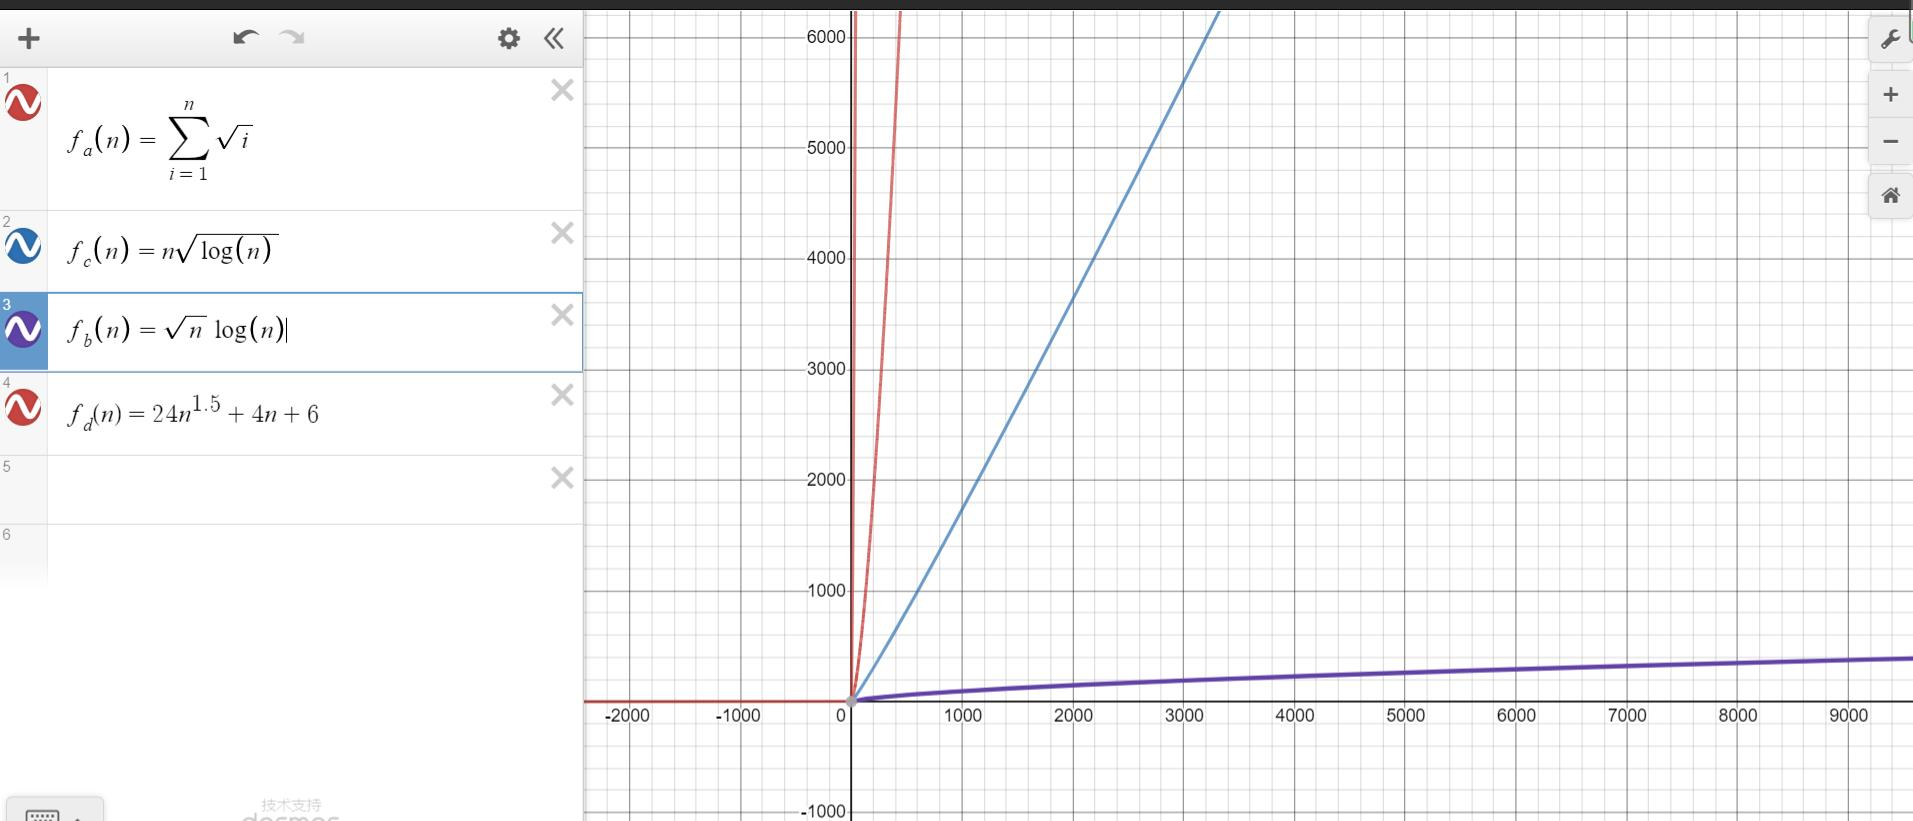
\includegraphics[scale=0.3]{hw104.jpg}
    \caption{Comparison}
\end{figure}
\\$f_b(n)<f_c(n)<f_a(n)<f_d(n)$

\section{Master Theorem}
\maketitle {1.a}
\\\\
\begin{forest}
[$f(n)$
    [$f(n/b)$
        [$f(n/b^2)$[$\Theta (1)$][$\Theta (1)$]] 
        [$f(n/b^2)$[$\Theta (1)$][$\Theta (1)$]]
    ]    
    [$f(n/b)$
        [$f(n/b^2)$[$\Theta (1)$][$\Theta (1)$]]
        [$f(n/b^2)$[$\Theta (1)$][$\Theta (1)$]]
    ]
]
\end{forest}
This recursion tree will have $a$ branches, which means $a$ subnodes, depth 1 is $f(n/b)$, but also $af(n/b)$, total depth is $\log_b n$, the last $\Theta (1)$ is also $\Theta (n^{\log_b a})$.

\section{Ramanujam numbers}
\maketitle{1.}
\begin{algorithm}
    \caption{Ramanujam numbers}
    \begin{algorithmic}[1]
    \Require $n$
    \Ensure $Ramanujam\ numbers \leq n$
    \Function{$Ram$}{$n$}
    \State $i = 1,l = [\ ]$
    \While{$i \leq n$}
    \State intcount = 0
    \For {$j \in (1,i^{1/3})$}
    \For {$k \in (j+1,i^{1/3})$}
    \If {$j^3 + k^3 = i$}
    \State intcount $\gets$ intcount + $1$
    \EndIf 
    \EndFor
    \EndFor
    \If{intcount $\geq $ 2}
    \State $l \gets l + i$
    \EndIf
    \State $i \gets i+1$
    \EndWhile
    \State \Return $l$
    \EndFunction
    \end{algorithmic}
\end{algorithm}
The complexity should be $ O(n*n^{1/3}*n^{1/3})=O(n^{5/3})$
\\
\\
\\
\section{Critical Thinking}
\maketitle{1.}
\\Name those pirates P1, P2, P3, P4, P5, and P6, while P6 is the first one to propose and P1 be the last.
\\\\Start with P1 and P2, at this time P2 get whatever he proposed, so he'll choose all 300 coins for himself and poor have nothing to do with it.
\\\\And here comes P3, if he wants to get a 2:1, he'll choose P1 to be his teammate, so 1 coin for him, to vote agree for this design, the proposal will be \{299, 0, 1\} for P3, P2, and P1.
\\\\As for P4, He needs another voter to get 50\%. If his proposal is denied, then P3 will win, and P2 get nothing, so P4 should send a coin to P2, the proposal will be \{299, 0, 1, 0\} for P4, P3, P2, and P1.
\\\\If P4's proposal wins, P3 and P1 will get nothing. P5 then comes up with a new idea to let himself win, The proposal will be \{298, 0, 1, 0, 1\}.
\\\\Then P6 should come up with a same one, but give coins to different people to get 50\% upvote, The final proposal will be \{298, 0, 1, 0, 1, 0\} For P6, P5, P4, P3, P2, and P1.
\end{document}
